% This is "sig-alternate.tex" V2.1 April 2013
% This file should be compiled with V2.5 of "sig-alternate.cls" May 2012
%
% This example file demonstrates the use of the 'sig-alternate.cls'
% V2.5 LaTeX2e document class file. It is for those submitting
% articles to ACM Conference Proceedings WHO DO NOT WISH TO
% STRICTLY ADHERE TO THE SIGS (PUBS-BOARD-ENDORSED) STYLE.
% The 'sig-alternate.cls' file will produce a similar-looking,
% albeit, 'tighter' paper resulting in, invariably, fewer pages.
%
% ----------------------------------------------------------------------------------------------------------------
% This .tex file (and associated .cls V2.5) produces:
%       1) The Permission Statement
%       2) The Conference (location) Info information
%       3) The Copyright Line with ACM data
%       4) NO page numbers
%
% as against the acm_proc_article-sp.cls file which
% DOES NOT produce 1) thru' 3) above.
%
% Using 'sig-alternate.cls' you have control, however, from within
% the source .tex file, over both the CopyrightYear
% (defaulted to 200X) and the ACM Copyright Data
% (defaulted to X-XXXXX-XX-X/XX/XX).
% e.g.
% \CopyrightYear{2007} will cause 2007 to appear in the copyright line.
% \crdata{0-12345-67-8/90/12} will cause 0-12345-67-8/90/12 to appear in the copyright line.
%
% ---------------------------------------------------------------------------------------------------------------
% This .tex source is an example which *does* use
% the .bib file (from which the .bbl file % is produced).
% REMEMBER HOWEVER: After having produced the .bbl file,
% and prior to final submission, you *NEED* to 'insert'
% your .bbl file into your source .tex file so as to provide
% ONE 'self-contained' source file.
%
% ================= IF YOU HAVE QUESTIONS =======================
% Questions regarding the SIGS styles, SIGS policies and
% procedures, Conferences etc. should be sent to
% Adrienne Griscti (griscti@acm.org)
%
% Technical questions _only_ to
% Gerald Murray (murray@hq.acm.org)
% ===============================================================
%
% For tracking purposes - this is V2.0 - May 2012

\documentclass{sig-alternate-05-2015}
\usepackage{caption}
\usepackage{multirow}
\usepackage{float}
\usepackage{subcaption}
\usepackage{url}
\usepackage{graphicx}
\usepackage{epstopdf}
\graphicspath{{./figures/}}
\usepackage{color}
\usepackage[utf8]{inputenc}




\begin{document}
% Copyright
%\setcopyright{acmcopyright}
%\setcopyright{acmlicensed}
%\setcopyright{rightsretained}
%\setcopyright{usgov}
%\setcopyright{usgovmixed}
%\setcopyright{cagov}
%\setcopyright{cagovmixed}


% DOI
%\doi{10.475/123_4}

% ISBN
%\isbn{123-4567-24-567/08/06}

%Conference
%\conferenceinfo{PLDI '13}{June 16--19, 2013, Seattle, WA, USA}

%\acmPrice{\$15.00}

%
% --- Author Metadata here ---
%\conferenceinfo{KDD'16}{'97 El Paso, Texas USA}
%\CopyrightYear{2007} % Allows default copyright year (20XX) to be over-ridden - IF NEED BE.
%\crdata{0-12345-67-8/90/01}  % Allows default copyright data (0-89791-88-6/97/05) to be over-ridden - IF NEED BE.
% --- End of Author Metadata ---

\title{EMBERS Experiences}
%Format\titlenote{(Produces the permission block, and
%copyright information). For use with
%SIG-ALTERNATE.CLS. Supported by ACM.}}
%\subtitle{[Extended Abstract]
%\titlenote{A full version of this paper is available as
%\textit{Author's Guide to Preparing ACM SIG Proceedings Using
%\LaTeX$2_\epsilon$\ and BibTeX} at
%\texttt{www.acm.org/eaddress.htm}}}
%
% You need the command \numberofauthors to handle the 'placement
% and alignment' of the authors beneath the title.
%
% For aesthetic reasons, we recommend 'three authors at a time'
% i.e. three 'name/affiliation blocks' be placed beneath the title.
%
% NOTE: You are NOT restricted in how many 'rows' of
% "name/affiliations" may appear. We just ask that you restrict
% the number of 'columns' to three.
%
% Because of the available 'opening page real-estate'
% we ask you to refrain from putting more than six authors
% (two rows with three columns) beneath the article title.
% More than six makes the first-page appear very cluttered indeed.
%
% Use the \alignauthor commands to handle the names
% and affiliations for an 'aesthetic maximum' of six authors.
% Add names, affiliations, addresses for
% the seventh etc. author(s) as the argument for the
% \additionalauthors command.
% These 'additional authors' will be output/set for you
% without further effort on your part as the last section in
% the body of your article BEFORE References or any Appendices.
\numberofauthors{1} %  in this sample file, there are a *total*
% of EIGHT authors. SIX appear on the 'first-page' (for formatting
% reasons) and the remaining two appear in the \additionalauthors section.
%
\author{
% You can go ahead and credit any number of authors here,
% e.g. one 'row of three' or two rows (consisting of one row of three
% and a second row of one, two or three).
%
% The command \alignauthor (no curly braces needed) should
% precede each author name, affiliation/snail-mail address and
% e-mail address. Additionally, tag each line of
% affiliation/address with \affaddr, and tag the
% e-mail address with \email.
%
%\alignauthor
%\affaddr{Author List TBD} \\  %\titlenote{Dr.~Trovato insisted his name be first.}\\
%      \affaddr{Somwhere, Sometime}
%      \email{some1@somewhere.edu}
% uncommenting the triple comments will give you a rough approx of an author
% list
\alignauthor
 %\titlenote
  Sathappan Muthiah\footnotemark[1],
  Patrick Butler\footnotemark[1],
  Rupinder Khandpur\footnotemark[1],
  Prithwish Chakraborty\footnotemark[1],\\
  Saurav Ghosh\footnotemark[1],
  Parang Saraf\footnotemark[1],
  Nathan Self\footnotemark[1], 
  Liang Zhao\footnotemark[1],
  Jose Cadena\footnotemark[1],\\
  Theodoros Rekatsinas\footnotemark[2],
  Chang-Tien Lu\footnotemark[1],
  Bert Huang\footnotemark[1],
  Anil Vullikanti\footnotemark[1],\\
  Achla Marathe\footnotemark[1],
  Madhav Marathe\footnotemark[1],
  Lise Getoor\footnotemark[3],
  Kristen Summers\footnotemark[8],\\
  Graham Katz\footnotemark[8],
  Andy Doyle\footnotemark[4],
  Jaime Arredondo\footnotemark[6],
  Dipak Gupta\footnotemark[7],
  David Mares\footnotemark[6],\\
  Naren Ramakrishnan\footnotemark[1],
\\
\affaddr{\footnotemark[1]~~Virginia Tech}\\
\affaddr{\footnotemark[2]~~University of Maryland, College Park, MD 20742}\\
\affaddr{\footnotemark[3]~~University of California at Santa Cruz, Santa Cruz, CA 95064}\\
\affaddr{\footnotemark[8]~~~IBM Inc.}\\
\affaddr{\footnotemark[6]~~University of California at San Diego, San Diego, CA 92093}\\
\affaddr{\footnotemark[7]~~~San Diego State University, San Diego, CA 92182} \\
\affaddr{\footnotemark[5]~~BASIS Technology, Herndon, VA 20171}\\
\affaddr{\footnotemark[4]~~CACI Inc., Lanham, MD 20706}\\
}
\maketitle
\begin{abstract}
This paper gives an account of the successful forecasts made by the
EMBERS system and reasons out cases where EMBERS didnt perform well.
\end{abstract}


%%
%% The code below should be generated by the tool at
%% http://dl.acm.org/ccs.cfm
%% Please copy and paste the code instead of the example below. 
%%
%\begin{CCSXML}
%<ccs2012>
 %<concept>
  %<concept_id>10010520.10010553.10010562</concept_id>
  %<concept_desc>Computer systems organization~Embedded systems</concept_desc>
  %<concept_significance>500</concept_significance>
 %</concept>
 %<concept>
  %<concept_id>10010520.10010575.10010755</concept_id>
  %<concept_desc>Computer systems organization~Redundancy</concept_desc>
  %<concept_significance>300</concept_significance>
 %</concept>
 %<concept>
  %<concept_id>10010520.10010553.10010554</concept_id>
  %<concept_desc>Computer systems organization~Robotics</concept_desc>
  %<concept_significance>100</concept_significance>
 %</concept>
 %<concept>
  %<concept_id>10003033.10003083.10003095</concept_id>
  %<concept_desc>Networks~Network reliability</concept_desc>
  %<concept_significance>100</concept_significance>
 %</concept>
%</ccs2012>  
%\end{CCSXML}

%\ccsdesc[500]{Computer systems organization~Embedded systems}
%\ccsdesc[300]{Computer systems organization~Redundancy}
%\ccsdesc{Computer systems organization~Robotics}
%\ccsdesc[100]{Networks~Network reliability}


%%
%% End generated code
%%

%%
%%  Use this command to print the description
%%
%\printccsdesc

%% We no longer use \terms command
%%\terms{Theory}

\keywords{ACM proceedings; \LaTeX; text tagging}

%%main
\section{Introduction}
Modern communication forms such as social media and microblogs are not only rapidly
advancing our understanding of the world but also improving the methods by which we can 
comprehend, and even forecast, the progression of events.
Tracking population-level activities via `massive passive' data has been shown to 
quite accurately shed light into large-scale societal movements. 

Two years back, in KDD 2014, we described EMBERS~\cite{beatingthenews-kdd}, a deployed anticipatory
intelligence system~\cite{bigdata-andy-doyle-embers-paper} that forecasts significant 
societal events (e.g., civil unrest
events such as protests, strikes, and `occupy' events) using a large set of open source
indicators such as news, blogs, tweets, food prices, currency rates, and other public
data. The EMBERS system has been running continuosuly 24x7 for nearly 4 years at this point
and our goal in this paper is to present the discoveries it has enabled,
correct as well as missed
forecasts, and lessons learnt from participating in a forecasting tournament including
our perspectives on the limits of forecasting and ethical considerations. In
particular, we shed insight into the value proposition to an analyst and how EMBERS forecasts
are communicated to its end-users. 

The development of EMBERS is supported by the Intelligence Advanced Research Projects
Activity (IARPA) Open Source Indicators (OSI) program. 
EMBERS forecasts are scored against the GSR (Gold Standard Report), a monthly catalog of 
events as reported in newspapers of record in the above countries. The GSR is compiled by MITRE corporation
using human analysts.
EMBERS currently focuses on multiple regions of the world but for the purpose of this paper
we focus primarily on Latin America, specifically the countries of
Argentina, Brazil, Chile, Colombia, Ecuador, El Salvador, Mexico, Paraguay, Uruguay, and Venezuela.
Similarly, EMBERS generates forecasts for multiple event classes---infleunza like illnesses~\cite{prithwish-ili},
rare diseases~\cite{sdm-saurav}, elections~\cite{aravindan-wei-besc}, domestic political crises~\cite{gdelt-acm-webscience}, and civil unrest---but in this paper we focus primarily on civil unrest as this was the
most challenging event class with hundreds of events every month across the countries studied here.

Our key contributions can be summarized as follows:
\narenc{Refer to sections in each bullet.}
\begin{enumerate}
\item Unlike retrospective studies of predictability, EMBERS forecasts are communicated in real-time before the
event to MITRE/IARPA and scored independently of the authors. 
We present multiple quantiative indicators of EMBERS performance 
as well as insights into how
we made EMBERS forecasts most valuable to analysts. We report two primary
ways in which analysts utilize EMBERS and the use of {\it automated
narratives} to help make EMBERS forecasts as useful as possible.

\item In an attempt to demystify the state-of-the-art
in forecasting and create an open dialogue in the community, we report both successful
forecasts of EMBERS as well as events missed by EMBERS. The events not forecast by EMBERS lead us to
considerations of both limitations of the underlying technology as well as inherent limits to
forecasting large-scale events.
\item While social media is often touted as key to event forecasting
systems such as EMBERS, we present the results of an ablation study to outline
the performance degradation that ensues if data sources 
such as Twitter and Facebook were to be removed from the forecasting pipeline.
\item We consider the separation of civil unrest events into events
that happen with a degree of regularity versus rare
or significant
events, and evaluate the performance of EMBERS in forecasting such
surprising events.
\item We describe our current best understanding of the limitations to
forecasting civil unrest events using technologies like EMBERS and 
also ethical considerations.
\end{enumerate}



%%civilunrest
\section{Civilunrest Forecasting}
The following section details out some of the successful and not so
successful forecasts made by EMBERS over the past few years in Latin America.
\subsection{Successful Forecasts}
Described below are some examples of successful civilunrest
forecasts made by the EMBERS system during 2013-2015.

\textbf{Brazil Spring (June 2013)}: These protests were the largest and most
significant protests in Brazil`s recent history that caught worldwide
attention. Millions of Brazilians took part in these demonstrations,
also known as the Brazilian Spring or the Vinegar Movement (inspired
from the use of vinegar soaked cloth by demonstrators to protect
themselves from police teargas), which were catalyzed by an increase in
public transport fares from $R\$3$ to $R\$3.20$ by the government of President
Dilma Rousseff.

As shown in Figure.~\ref{fig:brazilJune13} EMBERS, while missing the initial uptick,
captured the increase in the order of magnitude of the protest events
during the Brazilian Spring and also captured
the spatial spread in the events, in addition to forecasting that this would be
a "General Population" protest.

\begin{figure}[H]
\centering
\includegraphics[width=.8\columnwidth]{cu/brazilJune13}
\caption{Brazil Spring}
\label{fig:brazilJune13}
\end{figure}

Around 68\% of EMBERS Brazil alerts resulted from detected planned
protest which can be explained from the fact that the social networking
sites (Twitter and Facebook) and conventional news media played a key
role in organization of these uprisings. Although, initial protests were
mostly against the bus fare increase soon these grew from general
population's deep dissatisfactions to include wider issues such as -
government corruption, over-spending and police brutality. Also,
demonstrators made calls for political reforms. In response, President
Rousseff proposed a referendum on widespread political reforms in
Brazil, but was later abandoned. EMBERS models were able to capture such
discussions on Twitter (see Figure.~\ref{fig:brazilJune13_wordCloud}), and followed these stories as
they evolved through June.

\begin{figure}[H]
\centering
\includegraphics[width=.8\columnwidth]{cu/brazilJune13_wordCloud}
\caption{Word cloud from data extracted by EMBERS models}
\label{fig:brazilJune13_wordCloud}
\end{figure}

The protests intensified in late June (see Figure.~\ref{fig:brazilJune13}), which were
captured by EMBERS, as they also coincided with FIFA 2013 Confederations
Cup matches. This was an important factor due to which protests gained
momentum as they were covered by world media. Majority of protests
occurred in those cities, which were hosting (FIFA) soccer matches.
EMBERS submitted most of its alerts for these host cities (see Figure
~\ref{fig:brazilJune13_map}){\textemdash} Rio de Janeiro, São Paulo,
Belo Horizonte, Salvador and Porto Alegre,
among others. For example, on 27th June during Confederations cup
semi-final in Fortaleza, around 5000 protestors clashed with the police
near the Castelao stadium - In this case EMBERS sent out an alert the
day before. Then later on 30th June, when the last games of the
confederation cup took place in Rio de Janeiro and Salvador that were
also plagued by mass protests – EMBERS predicted these events and
submitted multiple alerts for Rio on 28th and 29th June and one for
Salvador on 29th June.

\begin{figure}[H]
\centering
\includegraphics[height=.6\columnwidth]{cu/brazilJune13_map}
\caption{Geographic overlap of Groud Truth protest events and EMBERS
alerts for Brazil June 2013.}
\label{fig:brazilJune13_map}
\end{figure}

\textbf{Venezuelan Spring (Feb-March 2014)}:
EMBERS captured some of the first `calls to protest` for the trigger city of
San Cristobal and its nearby surrounding areas and correctly forecast the
population (Education) and that the protests would turn violent. Over the next
days, EMBERS closely forecast the spike in the number of events as shown
in Figure.~\ref{fig:venezuelaMarch14} and the spread
of the protests to additional cities as shown in
Figure.~\ref{fig:venezuelaMap}.

\begin{figure}[H]
\centering
\includegraphics[width=.8\columnwidth]{cu/venezuelaFeb14}
\caption{Venezuelan Spring}
\label{fig:venezuelaMarch14}
\end{figure}

\begin{figure}[H]
\centering
\includegraphics[width=.6\columnwidth]{cu/venezuelaMap}
\caption{Venezuelan Spring}
\label{fig:venezuelaMap}
\end{figure}

\textbf{Mexico Protests (October 2014)}:
EMBERS , as shown in Figure.~\ref{fig:mexicoOct14} forecast an uptick of Mexico
protests during early October 2014 stemming from students and teachers demanding
action on the 43 students missing case, with a lead time of about 3
days. It also generated  a series of alert spikes coinciding with the first
large-scale nationwide protests between October 5th to 8th.

\begin{figure}[H]
\centering
\includegraphics[width=.8\columnwidth]{cu/mexicoOct14}
\caption{Mexico Protests}
\label{fig:mexicoOct14}
\end{figure}

Figure.~\ref{fig:mexicoTimeline} provides a timeline of GSR events and
EMBERS alerts for Mexico during this period
\begin{figure}[H]
\centering
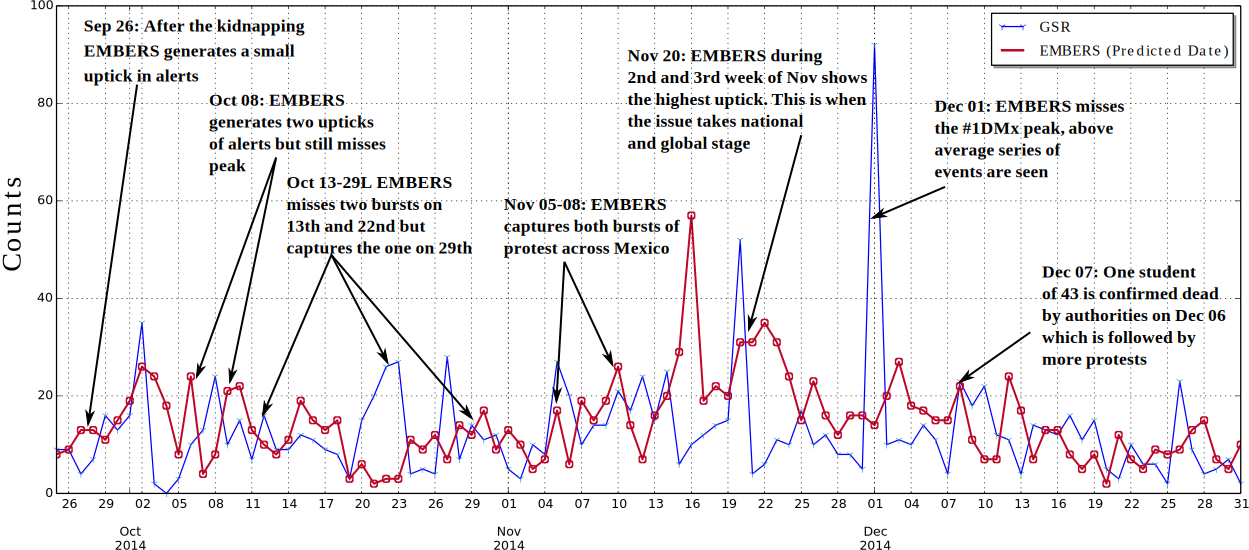
\includegraphics[width=.8\columnwidth]{cu/mx_timeline}
\caption{Mexico Protest timeline.The plot indicates the comparison between counts of GSR events
and EMBERS alerts’ for unique states/admins per day.The  }
EMBERS series’ as can be seen is more pronounced during Nov-Dec’14,
\label{fig:mexicoTimeline}
\end{figure}

\textbf{Colombia Protests (December'14 -March'15)}:
EMBERS successfully forecast the uptick in the number of events during the
middle of December 2014 and also the increase in protest counts during February
2015 as shown in Figure.~\ref{fig:colombiaDec14}, though in the latter case EMBERS over predicted the counts. The uptick in
December 2014 was led by the opposition leader Alvaro Uribe against impunity.
Whereas the increase in  protest counts in February 2015
was due to trucker’s strike against increase in fuel price.

\begin{figure}[H]
\centering
\includegraphics[width=.8\columnwidth]{cu/colombiaDec15}
\caption{Colombia Protests}
\label{fig:colombiaDec14}
\end{figure}

\textbf{Paraguay Protests (February 2015)}:
EMBERS forecast the uptick in number of protest events in Paraguay during mid
February 2015 as shown in Figure.~\ref{fig:paraguay15}. The events were mainly due to the lack of opportunity and basic
needs and against the introduction of new public-private partnership law.

\begin{figure}[H]
\centering
\includegraphics[width=.8\columnwidth]{cu/paraguayFeb15}
\caption{Paraguay Protests}
\label{fig:paraguay15}
\end{figure}


\subsection{Events missed by EMBERS}:
The following section details out certain events that EMBERS failed to
capture properly.

\textbf{Brazil Protests (March 2015)}: EMBERS predicted the accurate
increase in the rate of events but does not capture the true counts. The
protests were mainly targeted against president Dilma Rousseff due to
increasing corruption. 

During this period there was a significant architectural change in the
EMBERS processing pipeline. EMBERS had moved to Heideltime temporal
tagger from the previously used TIMEN temporal tagger due to
Heideltime`s support for more languages and active development cycle as
opposed to TIMEN. Heideltime had no support for portuguese (the main
language used in Brazil) and EMBERS team had extended Heideltime to
portuguese by translating the resources for spanish to portuguese. It
turned out that simple translation of rules from spanish to portuguese
were not sufficient and this affected the recall of one of our main
models for Brazil - Planned Protest - as it depended on the quality and recall of
date extraction from text.

\begin{figure}[H]
\centering
\includegraphics[width=.8\columnwidth]{cu/brazilMarch15}
\caption{Brazil 2015 Protests}
\label{fig:brazilSpring}
\end{figure}


\textbf{Mexico December 1, 2014 Protests}:
EMBERS missed the huge single day spike on December 1st when
people turned out in huge numbers in different parts of Mexico demanding
Pena Nieto`s ouster.
EMBERS predicted nationwide events for December 1st but failed to
capture the its spread. 

December 1st was picked by the protestors due to
its historical significance - it was the day when Pena Nieto was sworn
in as President in 2012 amidst much controversy and opposition from
general public. Also another reason for the missed prediction was due to 
EMBERS inability in extracting dates mentioned using twitter lingo  like "\#1Dmx".

\subsection{Surprising Events Predicted by EMBERS}To rigorously evaluate the capabilities of EMBERS, we implemented a baserate model as a yardstick for comparison. The baserate model generates alerts using the rate of occurrence of events in the past three months. While such a model will perform well when the average number of events per month doesn't fluctuate much, it will miss out predictions when there are sudden wide-spread nationwide protest events. 


In order to identify surprising events, we employed a Maximum Entropy Based Approach. For this approach, each event is described using the following three dimensions: Country, Population and Event Type. A three-dimensional cuboid as shown in figure ~\ref{fig:maxent_model} succinctly captures the event distribution across the three dimensions. In the Maximum Entropy Approach, Maximum Likelihood Estimates for each cell of this cuboid is generated while keeping the marginals constant. For any given month, deviations from these MLE estimates are calculated and the cells with maximum deviations are termed as `surprising events cell'.

\begin{figure}[H]
\centering
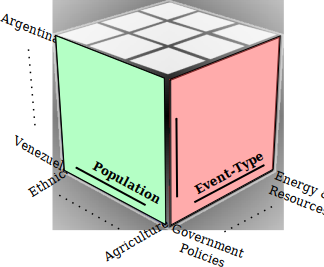
\includegraphics[width=.7\columnwidth]{cu/maxent_model}
\caption{Maximum Entropy Counts Cuboid}
\label{fig:maxent_model}
\end{figure}

Every month, events from the last three months of GSR is used to populate this event distribution cuboid. Once the cuboid is populated, we apply Iterative Proportional Fitting Procedure\cite{ipfp} to estimate the Maximum Likelihood values for each cell while keeping the marginals constant. The resultant cuboid is then scaled to matched the number of events in the current month. A similar three-dimensional cuboid is generated for the events of the current month and difference is calculated between actual counts and scaled MLE counts for each cell. Subsequently, all the cells with difference greater that 5-sigma are classified as `surprising' and events corresponding to these cells are used to generated a smaller version of GSR called `Surprising GSR'. 

\subsubsection{Iterative Proportional Fitting Procedure (IPFP)}
IPFP was invented in 1940's by Deming and Stephan\cite{deming1940least}. It is used to obtain Maximum Likelihood Estimates for the elementary cells by iterative fitting of the sufficient configurations. The procedure for a three dimensional structure, described in much detail in \cite{bishop2007discrete}, proceeds as follows:
\begin{enumerate}
\item Once the marginals are identified, elementary cells are replaced by 1; $\widehat{m}^{(0)}_{ijk}=1$
\item After initialization, the following three-step iterative cycle is performed till a satisfactory stopping goal is achieved:
$$\widehat{m}^{(c+1)}_{ijk} = \widehat{m}^{(c)}_{ijk}\frac{x_{ij+}}{\widehat{m}^{(c)}_{ij+}}$$
$$\widehat{m}^{(c+2)}_{ijk} = \widehat{m}^{(c+1)}_{ijk}\frac{x_{i+k}}{\widehat{m}^{(c+1)}_{i+k}}$$
$$\widehat{m}^{(c+3)}_{ijk} = \widehat{m}^{(c+2)}_{ijk}\frac{x_{+jk}}{\widehat{m}^{(c)}_{+jk}}$$
where c refers to iteration cycle and `+' refers to summation over a dimension. 
\item The procedure stops if either the desired convergence of $\delta < 0.0001$ is achieved or the maximum number of iterations are reached.
\end{enumerate}


\begin{table}
\caption{List of Nation-wide Events}
\renewcommand{\arraystretch}{1.1}
\vspace{-3mm}
 \centering
 \begin{tabular}{|l|l|m{6cm}|}
 \hline
May'13  &  Colombia	 &  Nationwide protests against administrative policy changes regarding Youth in Action program and Social Security Pension \\ \hline
Jun'13  &  Brazil  &  Brazilian Spring \\ \hline
Jul'13  &  Brazil  &  Brazilian Spring \\ \hline
Sep'13  &  Mexico  &  Nationwide protests Against Education and Energy Reforms \\ \hline
Oct'13  &  Mexico  &  Nationwide protests Against Education and Energy Reforms \\ \hline
Oct'13  &  Uruguay  &  Nationwide protests demading increase in minimum wage \\ \hline
Feb'14  &  Venezuela	  &  Venezuelan Spring \\ \hline
Mar'14  &  Venezuela  &  	Venezuelan Spring \\ \hline
May'14  &  Brazil  &  Nationwide demonstrations in response to the 2014 FIFA World Cup and other Social Issues \\ \hline
Jun'14  &  Brazil  &  Nationwide demonstrations in response to the 2014 FIFA World Cup and other Social Issues \\ \hline
Aug'14  &  Argentina	  &  Nationwide protests against fall in wages, employment and inflation \\ \hline
Sep'14  &  Ecuador  &  Nationwide protests to demand changes in labor policies \\ \hline
Oct'14  &  Mexico  &  Nationwide protests because of the discovery of Mass Grave of Kidnapped Students  \\ \hline
\end{tabular}
\vspace{-5mm}
\label{tab:maxentEvents}
\end{table}


\subsubsection{Surprising Events Results}
In table~\ref{tab:maxentEvents} we present several such cases where sudden nationwide events erupted. For all these events, we compare the recall of both EMBERS and baserate model in figure ~\ref{fig:maxent}. While EMBERS is able to pick up `{indicators}' for these protest events, baserate model fails to deliver.

\begin{figure}[H]
\centering
\includegraphics[width=.99\columnwidth]{cu/maxent}
\caption{Recall comparison of Surprising Events}
\label{fig:maxent}
\end{figure}

\section{Influenza-like-Illness Forecasting}
In this section we analyze the forecasts generated for Influenza-like-Illness
or ILI events. For ILI, we concentrated on short-term forecasts for the first 
2 years of \EMBERS. We shited our focus to long-term forecasts for the subsequent
years. We analyze both types of forecast here for general performance and 
analyze in details a few succesful forecasts which showcased the strength 
our system. There were a number of \EMBERS~ILI forecasts which significantly
deviated from the target sources. We analyzed these scenarios and discuss in 
details some of the weakness of \EMBERS. These scenarios also helped us to 
increase the robustness of our system.

\prithwi{TODO:}
\begin{itemize}
  \item Histogram of short-term forecasts QS/lead time
  \item Histogram of long-term forecasts QS/lead time
  \item CI for all categories. -- signficance of bad/good forecasts.
\end{itemize}

\subsection{successes}
\prithwi{Long-term and short term}

\begin{figure*}[tb!]
  \subcaptionbox{}{\includegraphics[width=0.9\textwidth]{../figures/ili/narrative1.png}}
  \\
  \subcaptionbox{}{\includegraphics[width=0.9\textwidth]{../figures/ili/narrative3.png}}

  \caption{\label{} ILI short-term: success stories}
\end{figure*}

\begin{itemize}
  \item {\bf Short-term:} ILI case counts for Chile for event date 08/07/13.
    \begin{itemize}
      \item Actual value: 626
      \item First update: 581 (QS: 3.71)
      \item Second update: 619 (QS: 3.95)
      \item Possible reason: season occuring around same time, similar shape.
    \end{itemize}

  \item {\bf Long-term:} ILI seasonal predictions for Bolivia
    \begin{itemize}
      \item Total flu/SRV count
      \item Peak date for flu/SRV
    \end{itemize}
\end{itemize}

\subsection{failures}

\begin{itemize}
  \item {\bf Short-term:} ILI case counts for Argentina
    \begin{itemize}
      \item Seasonality?
    \end{itemize}
  \item {\bf Long-term:} ILI seaonal predictions for Mexico
    \begin{itemize}
      \item Shifts in seasons. 
    \end{itemize}
\end{itemize}



\section{Rare Disease Forecasting}

One of the key event classes studied in EMBERS included forecasting outbreaks of four rare diseases (hantaviurs, cholera, yellow fever and machupo) in 10 countries of Latin America. The rare disease model employed a corpus of publicly available health-related news articles from HealthMap (cite) to extract topics about the mentioned rare diseases and their corresponding spatio-temporal patterns. The spatial and temporal distributions of rare disease topics were then utilized by 1-class SVM (cite) as features to predict the emergence of a rare disease outbreak at a future time point. This prediction is generated for each individual source where source refers to the publisher of the news articles, e.g. "www.biobiochile.cl" a prominent source reporting disease outbreak news in Chile. We had 798 different news sources extracted from the HealthMap corpus. To combine the predictions of multiple news sources, we used a multiplicative weights algorithm (cite).


\subsubsection{Successful forecasts}

EMBERS rare disease model successfully forecasted the hantavirus outbreaks in Chile and Argentina (2013 and 2014).

\subsubsection{Failures}

EMBERS rare disease model failed to forecast the cholera outbreak in Mexico during the month of October, 2013. One of the possible reasons is that this cholera outbreak spread to Mexico from its neighboring country Cuba, thus there was no prior signal about this outbreak in the HealthMap corpus. Alternative data sources, such as travel patterns could have helped us in forecasting this outbreak.


\section{Conclusions}
This paragraph will end the body of this sample document.
Remember that you might still have Acknowledgments or
Appendices; brief samples of these
follow.  There is still the Bibliography to deal with; and
we will make a disclaimer about that here: with the exception
of the reference to the \LaTeX\ book, the citations in
this paper are to articles which have nothing to
do with the present subject and are used as
examples only.


\section*{Acknowledgments}
{\small Supported by the Intelligence Advanced Research Projects Activity (IARPA) via
DoI/NBC contract number D12PC000337, the US Government is authorized to reproduce and distribute reprints of
this work for Governmental purposes notwithstanding any copyright annotation thereon.
Aravind Srinivasan and Khoa Trinh were also supported in part by NSF Award CNS
1010789.
Disclaimer: The views and conclusions contained herein are those of the authors and should not be interpreted as necessarily representing the official policies or endorsements, either expressed or implied, of IARPA, DoI/NBC, or the US Government.
}
% The following two commands are all you need in the
% initial runs of your .tex file to
% produce the bibliography for the citations in your paper.
\bibliographystyle{abbrv}
\bibliography{references}  % sigproc.bib is the name of the Bibliography in this case
% You must have a proper ".bib" file
%  and remember to run:
% latex bibtex latex latex
% to resolve all references
%
% ACM needs 'a single self-contained file'!
%
%APPENDICES are optional
%\balancecolumns
%\appendix
%%Appendix A
%\section{Headings in Appendices}
%The rules about hierarchical headings discussed above for
%the body of the article are different in the appendices.
%In the \textbf{appendix} environment, the command
%\textbf{section} is used to
%indicate the start of each Appendix, with alphabetic order
%designation (i.e. the first is A, the second B, etc.) and
%a title (if you include one).  So, if you need
%hierarchical structure
%\textit{within} an Appendix, start with \textbf{subsection} as the
%highest level. Here is an outline of the body of this
%document in Appendix-appropriate form:
%\subsection{Introduction}
%\subsection{The Body of the Paper}
%\subsubsection{Type Changes and  Special Characters}
%\subsubsection{Math Equations}
%\paragraph{Inline (In-text) Equations}
%\paragraph{Display Equations}
%\subsubsection{Citations}
%\subsubsection{Tables}
%\subsubsection{Figures}
%\subsubsection{Theorem-like Constructs}
%\subsubsection*{A Caveat for the \TeX\ Expert}
%\subsection{Conclusions}
%\subsection{Acknowledgments}
%\subsection{Additional Authors}
%This section is inserted by \LaTeX; you do not insert it.
%You just add the names and information in the
%\texttt{{\char'134}additionalauthors} command at the start
%of the document.
%\subsection{References}
%Generated by bibtex from your ~.bib file.  Run latex,
%then bibtex, then latex twice (to resolve references)
%to create the ~.bbl file.  Insert that ~.bbl file into
%the .tex source file and comment out
%the command \texttt{{\char'134}thebibliography}.
%% This next section command marks the start of
%% Appendix B, and does not continue the present hierarchy
%\section{More Help for the Hardy}
%The sig-alternate.cls file itself is chock-full of succinct
%and helpful comments.  If you consider yourself a moderately
%experienced to expert user of \LaTeX, you may find reading
%it useful but please remember not to change it.
%%\balancecolumns % GM June 2007
%% That's all folks!
\end{document}
